%======================================================================
\section{Introduction}
%======================================================================

Whether receiving help on an online platform motivates subsequent helping behavior has been a persistent question in the study of online communities. Generalized reciprocity, the tendency to help others after being helped oneself \citep{nowak_upstream_2007, baker_paying_2014}, is among the mechanisms proposed to sustain cooperation on platforms like Stack Overflow and Wikipedia, where direct exchange between the same two individuals is rare. If receiving help reliably increases the probability of giving it, cooperation may sustain itself through cascading helping acts, even among strangers \citep{fowler_cooperative_2010}. The behavioral evidence, however, is inconsistent: some observational studies find substantial reciprocity effects \citep{baker_paying_2014, chen_why_2019}, while others find weak or null relationships \citep{wasko_why_2005, joyce_predicting_2006}. We argue that much of this inconsistency is methodological.

Observational studies of reciprocity on platforms face a persistent confound: more engaged users are more likely both to seek help and to provide it, regardless of whether their own questions are resolved. Studies that correlate help received with help given, without accounting for this baseline activity, conflate reciprocity with general user engagement \citep{baker_paying_2014, chen_engaging_2018, joyce_predicting_2006}. A related limitation is that prior designs have largely treated receiving help as a one-time event, even though help-seeking and helping occur continuously and in overlapping waves throughout a user's tenure.

We address both problems by developing a matched difference-in-differences survival analysis, applied to over 24 million question-level observations from Stack Overflow. For each question a user posts, we define observation windows before and after the question and compare changes in helping behavior between users whose question received an answer (treated) and propensity-score-matched users whose question did not (control). Matching on user tenure, activity history, and question characteristics makes the groups comparable on the observable predictors of receiving and giving help. A Cox proportional hazards framework accommodates the continuous-time dynamics of helping behavior and the staggered, time-varying structure of treatment.

We develop two theoretical predictions alongside the basic reciprocity hypothesis. Drawing on theories of socialization and norm internalization, we predict that the reciprocity effect is stronger among newcomers than among experienced users (H2). Newcomers have not yet internalized community-specific norms or learned to value platform incentives such as reputation points; general moral obligations to reciprocate are therefore more likely to drive their behavior. As users accumulate experience, these general-purpose triggers may be displaced by community-specific motivations. We also predict that faster responses should amplify the reciprocity effect (H3), on the grounds that gratitude is more intense when help arrives while the need is still salient \citep{mccullough_is_2001, tsang_gratitude_2006}.

The results support H1 and H2 but not H3. Receiving an answer increases the hazard of helping by roughly 12\% in the pooled sample (HR\,=\,1.12, $p < .001$). This effect declines monotonically across seven tenure buckets, from hazard ratios of approximately 1.14--1.15 among users with less than one month of tenure to approximately 1.05 among those with more than six years. The response time prediction is not supported. In the pooled data, the reciprocity effect follows an inverted-U: near zero for questions answered in under one hour, elevated at roughly 1.10--1.11 for questions answered in one to eight hours, and attenuating at longer delays. The stratified models reveal heterogeneity across experience levels: newcomers show a positive speed interaction (slower answers associated with slightly stronger effects, contrary to H3); users with one week to twelve months of tenure show no significant response time moderation; and established users show positive interactions of increasing magnitude, with the largest effects at longer response times.

We interpret the experienced-user pattern through what we call the \textit{re-engagement window}. Posting an unanswered question keeps users engaged with the platform while the request is pending; they remain active and encounter helping opportunities. A fast answer resolves the need and creates an exit cue, reducing the time spent on the platform and thereby suppressing the conditions for reciprocal helping. A very slow answer arrives after the user has disengaged and the question has faded in relevance. The effect is largest when the answer arrives in the intermediate range: after the user may have briefly stepped away, but while the question is still current enough to draw them back. Among newcomers, the session-exit dynamics appear weaker, though the precise mechanism underlying their positive speed interaction is harder to identify from our data. Descriptive evidence for the re-engagement account appears in Figure~\ref{fig:help_rate_adoption_pooled} and Appendix Figure~\ref{fig:help_rate_adoption_by_tenure}.

Our study makes three contributions. First, we provide evidence that receiving help on Stack Overflow increases subsequent helping, using an identification strategy that addresses the endogeneity problems present in prior work. Second, we show that this effect is concentrated among newcomers and substantially attenuated among experienced users, consistent with the view that reciprocity functions primarily as a contributor-recruitment mechanism rather than a driver of sustained helping. Third, we identify a re-engagement window through which platform session dynamics moderate the response time effect on reciprocity, a result that challenges the direct application of laboratory-based theories of emotional immediacy to task-driven field settings.

%======================================================================
\section{Theory}
%======================================================================

%----------------------------------------------------------------------
\subsection{Generalized Reciprocity}
%----------------------------------------------------------------------

A central mechanism proposed to support cooperation in online communities is \textit{generalized reciprocity}, the tendency for individuals who have received help to help others in turn even when the recipient is not the original benefactor, \citep{nowak_upstream_2007, fowler_cooperative_2010}. Unlike direct reciprocity, which involves returning favors to the same individual, generalized reciprocity requires no repeated interactions or exchange with the same person. Instead, it operates as a ``pay-it-forward'' model, sustaining collective contributions within groups where members may have infrequent or non-recurring interactions, such as online knowledge-sharing platforms.

Socio-psychological research identifies two complementary mechanisms underlying generalized reciprocity: moral reasoning and emotional responses. On the moral side, individuals may be guided by the logic of universalization \citep{levine_logic_2020}: they consider what would happen if all members requested more help than they gave. Such deliberation typically leads individuals to conclude that widespread free-riding would undermine the community as a valuable source of help, generating a shared moral obligation to reciprocate \citep{curry_is_2019}. This renders the relationship between individual and group into an indirect exchange: if one receives help from the group, one feels obligated to help the group in return.

Emotional mechanisms reinforce these moral considerations. A prominent response is gratitude, aroused by the perceived generosity of others \citep{mccullough_is_2001, mccullough_adaptation_2008}. Gratitude has been shown to motivate prosocial actions toward others independent of direct reciprocation \citep{tsang_gratitude_2006, bartlett_gratitude_2006}. According to \citet{molm_building_2007}, such emotional responses are especially important in systems where free riding is easy, such as on online knowledge-sharing platforms. Experiencing gratitude in these contexts not only increases the propensity to help but also strengthens perceptions of the community as valuable and worth sustaining \citep{elster_norms_2009}.

Generalized reciprocity is among the most widely studied behavioral mechanisms explaining cooperative behavior in groups, owing to its potential to initiate cascading acts of generosity \citep{fowler_cooperative_2010, boyd_evolution_1989}. Comparative research and meta-analyses indicate that it is a globally shared moral principle \citep{curry_is_2019}. Robust experimental evidence comes from both laboratory \citep{greiner_indirect_2005, molm_building_2007, stanca_measuring_2009} and field settings \citep{mujcic_indirect_2018, fowler_cooperative_2010}.

%----------------------------------------------------------------------
\subsection{Empirical Challenges in Measuring Generalized Reciprocity}
%----------------------------------------------------------------------

Despite its theoretical centrality, empirical findings on generalized reciprocity in online communities are mixed, and we argue that this inconsistency is largely attributable to persistent methodological challenges. Understanding these challenges is essential both for interpreting existing findings and for motivating our analytical approach.

A first challenge concerns the reliance on self-reported motives in surveys and interviews. Contributors frequently describe reciprocity as a central reason for their engagement \citep{wasko_it_2000, lakhani_how_2003}, yet sociological and psychological research has demonstrated that people have difficulty articulating the moral motives behind their actions \citep{vaisey_motivation_2009, mcclelland_how_1989}. When users state that they help because they enjoy it or feel a sense of obligation, it is unclear whether this reflects genuine reciprocity, altruism, conformity to perceived social norms, and the popular rhetoric of 'giving back', or post-hoc rationalization. The distinction between reciprocity and other prosocial motives, such as the intrinsic joy of helping or the pursuit of social status, is particularly difficult for individuals to make through introspection \citep{batson1991altruism, benabou_incentives_2006}. As a result, self-reported data might overstate the prevalence of reciprocity as a discrete motive.

A second and more fundamental challenge is the endogeneity of help-seeking and help-giving in observational data. Users who ask questions on platforms like Stack Overflow are also disproportionately likely to answer questions, not because receiving help triggered a reciprocal response, but because both behaviors reflect the same underlying characteristics, such as greater platform engagement. Studies that correlate help received with help given without accounting for this baseline activity effectively confound reciprocity with user type \citep{baker_paying_2014, chen_engaging_2018, joyce_predicting_2006}. As we discuss below, the confound between reciprocity and user type is the central identification challenge that motivates our matched diff-in-diff design.

Third, most studies of reciprocity employ cross-sectional designs that capture only a snapshot of motivational profiles at a single point in time. This makes it impossible to detect how reciprocity evolves as users gain experience on a platform. As we argue below, the strength of generalized reciprocity is not constant over the user trajectory but declines as users become socialized into community-specific norms. Cross-sectional analyses that pool newcomers with experienced users will conflate these heterogeneous effects, potentially masking the conditions under which reciprocity is most impactful.

%----------------------------------------------------------------------
\subsection{Reciprocity and the User Trajectory}
%----------------------------------------------------------------------

We propose that the mixed findings in the literature can be partly reconciled by attending to a dimension that prior research has largely overlooked: the user trajectory from newcomer to experienced contributor. We argue that generalized reciprocity is most potent early in a user's engagement and attenuates as users gain experience on the platform.

The logic of this prediction draws on theories of socialization and norm internalization. When a user first encounters an online community, they are unfamiliar with its specific norms, social structures, and reward systems. At this stage, community-specific incentives, such as reputation points, badges, or leaderboard positions, carry little motivational weight because the newcomer has not yet learned to value them. Instead, initial contributions are guided by more general moral principles that operate independently of community-specific knowledge. Generalized reciprocity is precisely such a principle: it requires only that the individual has received help and feels a moral obligation or emotional impulse to help in return, without any need to understand or identify with the particular community \citep{levine_logic_2020, curry_is_2019}.

As users interact with the community, they gradually learn its norms and develop a sense of membership. On platforms like Stack Overflow, these norms are codified in explicit reputation systems that reward helpful behavior with visible status markers. Once users internalize these community-specific norms, the broad moral obligation of reciprocity may be displaced by more localized incentive structures. The logic of universalization (``I should help because I was helped'') gives way to the logic of community membership (``I should help because that is what valued members do''). This norm displacement has been theorized in related contexts by \citet{benabou_incentives_2006}, who show how external incentives can crowd out moral motives.

Several additional mechanisms accelerate this decline. First, as users accumulate experiences of receiving help, each additional instance becomes less socially surprising and less likely to elicit strong gratitude \citep{mccullough_adaptation_2008}. The emotional response that fuels reciprocity habituates over time. Second, as users observe the platform's incentive structure that rewards helpful behavior with reputation and status, they may increasingly attribute others' helpful behavior to status pursuit rather than genuine generosity, further dampening the gratitude that triggers reciprocal helping.

This account predicts that generalized reciprocity is strongest among newcomers and declines with experience. This also helps explain why prior studies have reached different conclusions about the importance of reciprocity: those that focus on or oversample experienced users may underestimate reciprocity, while those that capture newcomer behavior may find stronger effects.

\hypmark{hyp:1}
\begin{quote}
\textsc{Hypothesis 1 (H1).} \emph{Receiving help increases a user's propensity to help others (generalized reciprocity effect).}
\end{quote}

\hypmark{hyp:2}
\begin{quote}
\textsc{Hypothesis 2 (H2).} \emph{The generalized reciprocity effect is strongest among newcomers and decreases as users gain experience on the platform.}
\end{quote}

%----------------------------------------------------------------------
\subsection{Response Time and the Immediacy of Reciprocity}
%----------------------------------------------------------------------

Having established predictions about the existence and trajectory of generalized reciprocity, we turn to a more fine-grained question: Does the speed of the helping experience matter? The emotional mechanisms underlying reciprocity suggest that it should. Gratitude, the primary emotional driver of generalized reciprocity \citep{mccullough_is_2001}, is an affective response that is triggered by the perception of a benefactor's generosity. The intensity of this emotional response is likely to depend on the characteristics of the helping experience, including its timeliness.

A swift response to a help request can amplify the experience of receiving help through several channels. First, a fast answer signals that the community is attentive and generous, strengthening the perception that the group is worth sustaining through reciprocal contributions. Second, gratitude is an emotional response that may be most intense when it is temporally proximate to the perceived need. When a user posts a question, their need for help is salient; a quick answer arrives during this window of heightened need. The longer the user waits for help, the less valuable the help is and the more likely they are to have gotten help elsewhere. Thus, quick responses are likely to intensify feelings of gratitude.

Conversely, delayed responses may attenuate reciprocity. When an answer arrives hours or days after the question was posted, the user's original need may have faded; they may have found a solution elsewhere, or the problem may have become less pressing. The interval between asking and receiving weakens the associative link between the two events, potentially diluting the emotional response. Furthermore, longer waits may signal that the community is less responsive or generous, weakening the perception that underpins the moral obligation to reciprocate.

These considerations lead to a straightforward prediction:

\hypmark{hyp:3}
\begin{quote}
\textsc{Hypothesis 3 (H3).} \emph{Faster responses to a user's question strengthen the generalized reciprocity effect, while slower responses weaken it.}
\end{quote}

We note that this hypothesis follows from the dominant theoretical accounts of generalized reciprocity, which emphasize emotional immediacy and the salience of the helping experience. However, as we will show, field settings introduce structural dynamics (particularly the behavioral consequences of session entry and exit on task-driven platforms) that can invert the predictions of laboratory-based theory. We return to this issue when presenting our results.

%======================================================================
\section{Empirical Setting: Stack Overflow}
\label{sec:empirical_setting}
%======================================================================

Stack Overflow offers a valuable empirical setting for examining generalized reciprocity in online knowledge sharing. The platform provides publicly available quarterly data dumps containing rich longitudinal information on user behavior, including knowledge-seeking and knowledge-providing activities dating back to the platform's inception. This extensive dataset enables the reconstruction of helping patterns over time, allowing for the analysis of temporal sequences of receiving and providing help, which is critical for studying generalized reciprocity. We note that Stack Overflow activity has declined in recent years, partly due to the rise of generative AI tools; however, the core question-and-answer dynamics we study are shared broadly across help forums and knowledge-sharing communities, supporting the generalizability of the mechanisms we identify.

At its core, Stack Overflow is a question-and-answer platform for software developers and technologists. As of mid-2025, the site had accumulated over 24 million questions and 36 million answers from more than 29 million registered users \citep{wikipedia_stack_overflow}. Its user base spans a wide range of experience levels and professional roles: the largest demographic group comprises developers aged 25--34, and the most common roles include full-stack, back-end, and front-end developers, along with a substantial share of students and those learning to code \citep{stack_overflow_developer_survey_2024}. Questions on the platform must be tightly focused on specific programming problems; broad or opinion-based inquiries are typically closed by community moderation \citep{stack_exchange_inc_how_2024}. The most frequently discussed topics, as reflected in question tags, include JavaScript, Python, Java, C\#, PHP, Android, and HTML, spanning areas from web development and mobile applications to data science and machine learning. Stack Overflow is built around several core features: tags categorize questions by topic, facilitating expertise matching; a voting system allows users to upvote or downvote questions and answers to assess quality; reputation points are earned for valued contributions such as providing high-quality answers; badges reward specific achievements; and bounties allow users to offer reputation points as rewards for helpful answers to particularly difficult questions \citep{stack_exchange_inc_how_2024}.

For our study, the key feature is the question-and-answer interaction between users. When a user posts a question, other users may provide answers, and the question author can mark one answer as ``accepted,'' indicating that the question has been resolved. This creates a clearly timestamped sequence (question posted, answer received) that we exploit to measure the temporal dynamics of generalized reciprocity. Crucially, on Stack Overflow, the identities of question-askers and answerers are typically different individuals, making this an ideal context for studying \textit{generalized} (rather than direct) reciprocity: users who receive help from one community member may subsequently help entirely different members.

%======================================================================
\section{Data and Methods}
\label{sec:methods}
%======================================================================

To test our predictions, we develop a matched staggered difference-in-differences survival analysis that leverages the temporal structure of help-seeking and help-giving on Stack Overflow. Our design compares changes in helping behavior (measured as the hazard of posting an answer) before and after a user receives an answer, between users who receive an answer and matched users who do not. This approach represents a novel integration of two methodological traditions: the staggered difference-in-differences framework of \citet{callaway_santanna_2021}, which accommodates variation in treatment timing and treatment effect heterogeneity, and the counting-process formulation of the Cox proportional hazards model \citep{andersen_gill_1982}, which allows treatment status and other covariates to vary continuously over the observation window.

%----------------------------------------------------------------------
\subsection{Study Design}
\label{sec:study_design}
%----------------------------------------------------------------------

For each question posted by a user, we construct a timeline centered on two key events: the posting of the question ($T_{\text{question}}$) and, for questions that receive an answer, the time at which the first qualifying answer is posted ($T_{\text{answer}}$). We define an observation window spanning the seven days before the question is posted ($T_{\text{question}} - 7\text{D}$) through the seven days after ($T_{\text{question}} + 7\text{D}$). This yields a 14-day timeline for each question, divided into distinct phases.

We define three phases within each observation window (see Figure~\ref{fig:study_design}):

\begin{enumerate}
    \item \textbf{Pre-question phase}: from the start of the observation window to the posting of the question ($T_{\text{question}} - 7\text{D}$ to $T_{\text{question}}$). This phase captures baseline helping activity before the focal question is asked.
    \item \textbf{Waiting period}: from the posting of the question to the receipt of the first answer ($T_{\text{question}}$ to $T_{\text{answer}}$). During this interval, the user has asked for help but has not yet received it.
    \item \textbf{Post-answer phase}: from the receipt of the answer to the end of the observation window ($T_{\text{answer}}$ to $T_{\text{question}} + 7\text{D}$). This is the phase in which the reciprocity effect, if it exists, should manifest.
\end{enumerate}

A key feature of our design is that units enter the post-answer (``treated'') phase at different elapsed times depending on how quickly they receive a response. This staggered entry into treatment is precisely the setting addressed by \citet{callaway_santanna_2021}, who show that standard two-way fixed-effects estimators can be biased when treatment timing varies and treatment effects are heterogeneous. Our approach avoids this pitfall by explicitly modeling the time-varying transition into treatment within each observation window and by comparing treated units only to not-yet-treated or never-treated controls.

For control users (those whose questions did not receive an answer), there is no natural transition between the waiting period and the post-answer phase. To maintain temporal alignment with the matched treated observation, we assign the control observation a synthetic phase transition at the same elapsed time as the treated user's response time. That is, if the treated user's answer arrived 4 hours after their question, the matched control observation's timeline is split at $T_{\text{question}} + 4\text{h}$, creating an aligned ``post'' phase of equal duration. This ensures that any differences between treated and control observations in the post-answer phase are not driven by differences in the length of the observation period. Throughout the paper, we use ``post-question'' to refer to the entire period after the question is posted, encompassing both the waiting period and the post-answer phase.

The survival clock in our Cox models is centered on the question-posting time: time zero corresponds to the start of the observation window ($T_{\text{question}} - 7\text{D}$), so that the question itself is posted at day~7 of the timeline and the observation window closes at day~14. All help events (answers posted by the focal user) are recorded with their exact timestamps and converted to elapsed time on this clock.

\begin{figure}[H]
\caption{Study Design: Matched Difference-in-Differences Survival Analysis}
\label{fig:study_design}
\centering
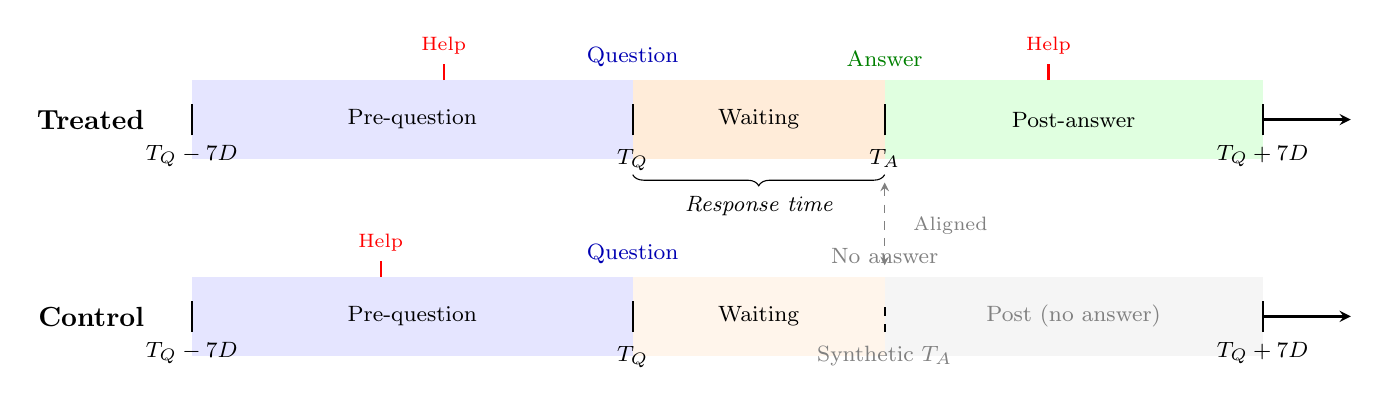
\begin{tikzpicture}[x=1.6cm, y=1cm, >=stealth, font=\small]

% --- Treated timeline ---
\node[anchor=east, font=\bfseries] at (-0.3, 2) {Treated};

% Main axis
\draw[thick, ->] (0,2) -- (9.2,2);

% Phase regions
\fill[blue!10] (0,1.5) rectangle (3.5,2.5);
\fill[orange!15] (3.5,1.5) rectangle (5.5,2.5);
\fill[green!12] (5.5,1.5) rectangle (8.5,2.5);

% Tick marks
\draw[thick] (0,1.8) -- (0,2.2);
\draw[thick] (3.5,1.8) -- (3.5,2.2);
\draw[thick] (5.5,1.8) -- (5.5,2.2);
\draw[thick] (8.5,1.8) -- (8.5,2.2);

% Labels below axis
\node[below, font=\footnotesize] at (0,1.8) {$T_Q - 7\text{D}$};
\node[below, font=\footnotesize] at (3.5,1.75) {$T_Q$};
\node[below, font=\footnotesize] at (5.5,1.75) {$T_A$};
\node[below, font=\footnotesize] at (8.5,1.8) {$T_Q + 7\text{D}$};

% Phase labels
\node[font=\footnotesize] at (1.75, 2) {Pre-question};
\node[font=\footnotesize] at (4.5, 2) {Waiting};
\node[font=\footnotesize] at (7.0, 2) {Post-answer};

% Response time brace
\draw[decorate, decoration={brace, amplitude=4pt, mirror}] (3.5, 1.3) -- (5.5, 1.3);
\node[below, font=\footnotesize\itshape] at (4.5, 1.15) {Response time};

% Question and answer markers
\node[above, font=\footnotesize, text=blue!70!black] at (3.5, 2.55) {Question};
\node[above, font=\footnotesize, text=green!50!black] at (5.5, 2.55) {Answer};

% --- Control timeline ---
\node[anchor=east, font=\bfseries] at (-0.3, -0.5) {Control};

% Main axis
\draw[thick, ->] (0,-0.5) -- (9.2,-0.5);

% Phase regions
\fill[blue!10] (0,-1) rectangle (3.5,0);
\fill[orange!8] (3.5,-1) rectangle (5.5,0);
\fill[gray!8] (5.5,-1) rectangle (8.5,0);

% Tick marks
\draw[thick] (0,-0.7) -- (0,-0.3);
\draw[thick] (3.5,-0.7) -- (3.5,-0.3);
\draw[thick, dashed] (5.5,-0.7) -- (5.5,-0.3);
\draw[thick] (8.5,-0.7) -- (8.5,-0.3);

% Labels below axis
\node[below, font=\footnotesize] at (0,-0.7) {$T_Q - 7\text{D}$};
\node[below, font=\footnotesize] at (3.5,-0.75) {$T_Q$};
\node[below, font=\footnotesize, text=gray] at (5.5,-0.75) {Synthetic $T_A$};
\node[below, font=\footnotesize] at (8.5,-0.7) {$T_Q + 7\text{D}$};

% Phase labels
\node[font=\footnotesize] at (1.75, -0.5) {Pre-question};
\node[font=\footnotesize] at (4.5, -0.5) {Waiting};
\node[font=\footnotesize, text=gray] at (7.0, -0.5) {Post (no answer)};

% Question marker
\node[above, font=\footnotesize, text=blue!70!black] at (3.5, 0.05) {Question};
\node[above, font=\footnotesize, text=gray] at (5.5, 0.05) {No answer};

% Alignment arrows
\draw[dashed, gray, <->] (5.5, 1.2) -- (5.5, 0.15);
\node[right, font=\scriptsize, text=gray] at (5.65, 0.65) {Aligned};

% Help events (example)
\draw[red, thick] (2.0, 2.5) -- (2.0, 2.7) node[above, font=\scriptsize, text=red] {Help};
\draw[red, thick] (6.8, 2.5) -- (6.8, 2.7) node[above, font=\scriptsize, text=red] {Help};
\draw[red, thick] (1.5, 0) -- (1.5, 0.2) node[above, font=\scriptsize, text=red] {Help};

\end{tikzpicture}

\vspace{0.5em}
\parbox{\textwidth}{\footnotesize\textit{Note.} Each observation window spans 14 days centered on the focal question ($T_Q$). The treated timeline (top) shows three phases: the pre-question phase (baseline), the waiting period (question posted, no answer yet), and the post-answer phase (after the first qualifying answer $T_A$ arrives). The control timeline (bottom) is from a propensity-score-matched user whose question did not receive an answer. To ensure temporal alignment, the control's post-question period is split at a synthetic transition point matching the treated user's response time. Red markers indicate help events (answers posted by the focal user to other users' questions). The treatment effect is identified as the differential change in helping hazard between treated and control observations in the post-answer phase, relative to the pre-question baseline. The staggered timing of $T_A$ across observations motivates our use of matched difference-in-differences methods robust to treatment effect heterogeneity \citep{callaway_santanna_2021}.}
\end{figure}

Within each timeline, we track all instances in which the user provides an answer to another user's question. These helping events constitute the outcome in our survival analysis. Conceptually, our design asks: Does the hazard of helping increase after a user receives an answer, relative to the change in hazard for a matched user who does not receive an answer? We present descriptive evidence on the raw help rates over this timeline in Section~\ref{sec:results} (Figure~\ref{fig:help_rate_2panel}), before turning to the formal Cox model estimates.

%----------------------------------------------------------------------
\subsection{Data}
%----------------------------------------------------------------------

We utilized the full sample of non-deleted questions from Stack Overflow's inception on 31 July 2008 through 1 April 2025. We addressed two edge cases that would render our fixed-length observation window invalid. First, for early platform questions, the pre-period could predate the platform's launch, meaning no answers were possible at that time. We removed 1,080 such cases. Second, due to the data dump's April~1, 2025, cut-off, the post-period could be prematurely truncated. We excluded 8,029 cases affected by this. We then excluded 2,671,121 questions that received an answer from the question poster. These filtering steps resulted in a pre-matching dataset of 21,033,429 questions from 4,764,048 unique users. After propensity score matching (described below), the final analytical dataset comprises 4,804,183 matched question-level observations from 908,775 unique users, with a 50\% treatment rate by construction.

%----------------------------------------------------------------------
\subsection{Variables}
%----------------------------------------------------------------------

Table~\ref{tab:variables} provides an overview of the variables used in our analysis. The phase terminology is consistent with Figure~\ref{fig:study_design}: the pre-question phase captures baseline behavior, the waiting period spans the interval from question to answer, and the post-answer phase captures the period after the answer arrives. We use ``post-question'' to refer to the combined waiting period and post-answer phase whenever distinguishing between these two sub-periods is not necessary.

\begin{table}[H]
\caption{Overview of Variables}
\label{tab:variables}
\centering
\begin{tabularx}{\textwidth}{@{}lX@{}}
\toprule
\textbf{Variable} & \textbf{Description} \\
\midrule
\multicolumn{2}{@{}l}{\textit{Outcome (Survival Event)}} \\
\hspace{1em} helpEvent & A binary event indicator equal to 1 at times when the user posts an answer to another user's question within the observation window. \\
\midrule
\multicolumn{2}{@{}l}{\textit{Time-Varying Covariates}} \\
\hspace{1em} phasePostQuestion & Binary; 1 for intervals occurring after the user posts their question ($t \geq T_{\text{question}}$), 0 otherwise. Captures the combined post-question period (waiting period + post-answer phase). \\
\hspace{1em} phasePostAnswer & Binary; 1 for intervals occurring after the user receives their first answer ($t \geq T_{\text{answer}}$), 0 otherwise. For control users (no answer received), this variable switches on at the synthetic transition point at the matched treated user's response time. Isolates the post-answer phase specifically. \\
\hspace{1em} treatedPostQuestion & Interaction of hasAnswer $\times$ phasePostQuestion; captures differential behavior of treated users in the entire post-question period (during the waiting period and beyond). \\
\hspace{1em} isTreatedActive & Interaction of hasAnswer $\times$ phasePostAnswer; the primary treatment effect capturing the additional lift in helping hazard after receiving an answer, beyond any change attributable to the act of asking a question. \\
\hspace{1em} treatedResponseTime & Interaction of isTreatedActive $\times$ $\widetilde{\log}(\text{RT})$; captures moderation of the post-answer treatment effect by answer speed. \\
\hspace{1em} treatedPostQuestionResponseTime & Interaction of treatedPostQuestion $\times$ $\widetilde{\log}(\text{RT})$; controls for moderation of the waiting-period effect by response time, ensuring the post-answer estimate $\gamma$ is not confounded by response-time-driven differences in waiting-period activity. \\
\bottomrule
\end{tabularx}
\end{table}

\paragraph{Outcome.} The event of interest in our survival analysis is the posting of an answer. Within each observation window, we track when (and whether) the focal user provides an answer to any other user's question. The Cox model estimates the instantaneous hazard of this helping event as a function of time-varying covariates that capture the phase of the observation timeline and the treatment status.

\paragraph{Treatment.} The treatment is the receipt of an answer. We operationalize this using \textit{hasAnswer}, a binary variable indicating whether the user's question received at least one answer with a non-negative score. We adopt this operationalization rather than Stack Overflow's ``accepted answer'' mechanism to address endogeneity: marking an answer as accepted requires the user to return to the site, which may itself correlate with helping behavior.

\paragraph{Response Time.} For each treated observation, the response time variable used in the interaction terms is $\log(1 + t_{\text{answer}})$, where $t_{\text{answer}}$ is the elapsed time in hours from the start of the observation window ($T_Q - 7\text{D}$) to the arrival of the first qualifying answer. Because $T_Q - 7\text{D}$ is a fixed origin common to all observations, this is a monotone transformation of the actual response time in hours ($t_{\text{answer}} - t_{\text{question}}$) and preserves the full ordering of fast versus slow answers; however, it shifts the scale by the constant pre-question window length. For numerical stability, both response-time interaction terms ($\text{isTreatedActive} \times \log(1+t_{\text{answer}})$ and $\text{treatedPostQuestion} \times \log(1+t_{\text{answer}})$) are clipped to their 5th--95th percentile range and then standardized (z-scored) before model fitting. Consequently, the reported interaction coefficients $\gamma$ and $\delta$ are expressed per one standard deviation of the respective interaction term rather than per unit of $\log(1+t_{\text{answer}})$.

\paragraph{User Experience.} To test Hypothesis 2, we stratify our analysis by user tenure, defined as the number of days between a user's first activity on the platform and the start of the observation window. We define seven tenure buckets using right-closed intervals: $[0, 7]$, $(7, 30]$, $(30, 180]$, $(180, 365]$, $(365, 1095]$, $(1095, 2190]$, and $(2190, \infty)$ days, corresponding to the labels less than one week, one week to one month, one to six months, six to twelve months, one to three years, three to six years, and more than six years, respectively. Running separate models by bucket enables us to examine how the reciprocity effect varies across the user trajectory without imposing a parametric functional form. Table~\ref{tab:tenure_counts} reports the number of matched observations and unique users in each bucket.

\begin{table}[H]
\caption{Sample Size by Tenure Bucket (Matched Dataset)}
\label{tab:tenure_counts}
\centering\small
\begin{tabular}{lrrr}\toprule
Tenure Bucket & Matched Obs.\ (Pairs) & Unique Users & \% of Total \\\midrule
$<$ 1 week       & 1,044,218 & 522,109 & 21.7\% \\
1 week -- 1 month  & 610,632  & 211,847 & 12.7\% \\
1 -- 6 months      & 936,480  & 188,439 & 19.5\% \\
6 -- 12 months     & 504,762  & 114,231 & 10.5\% \\
1 -- 3 years       & 802,944  & 142,608 & 16.7\% \\
3 -- 6 years       & 541,370  & 89,215  & 11.3\% \\
$>$ 6 years        & 363,777  & 61,434  & 7.6\% \\\midrule
\textbf{Total}     & \textbf{4,804,183} & \textbf{908,775} & \textbf{100\%} \\
\bottomrule
\end{tabular}

\vspace{0.3em}
\parbox{0.9\textwidth}{\footnotesize\textit{Note.} Matched observations counts are reported as pairs (treated + control). Unique users may appear across multiple tenure buckets if they posted questions at different stages of their platform career. All tenure buckets contain sufficient observations for stable estimation.}
\end{table}

%----------------------------------------------------------------------
\subsection{Propensity Score Matching}
\label{sec:matching}
%----------------------------------------------------------------------

Because the receipt of an answer (the treatment) is correlated with user characteristics (more experienced users, for instance, tend to ask higher-quality questions that are more likely to receive answers), we employ propensity score matching \citep{rosenbaum_rubin_1983} to improve the comparability of the treatment and control groups. Importantly, matching is performed \textit{across different users}: each treated question (from a user who received an answer) is matched to a control question (from a different user whose question did not receive an answer) that has a similar propensity to receive an answer based on observable pre-treatment characteristics. This cross-user matching ensures that treated and control observations are independent conditional on the matched covariates, while the difference-in-differences structure within each pair absorbs residual differences.

We estimate the propensity score using the following pre-treatment covariates, which jointly capture user experience, recent activity, and question characteristics as depicted in Table \ref{tab:covariates}. It should be noted that \textit{tagAnswerRateAvg} is critical for addressing the concern that question complexity may confound the treatment: questions in tags with low answer rates are inherently more difficult, and matching on this rate ensures that treated and control questions come from similarly tractable topic areas.
Matching on the tag-level answer rate is particularly important for our response time analysis, as it mitigates the concern that slower response times simply proxy for differently sized sub-communities with lower throughput. 

\begin{table}[H]
\caption{Definition of Matching Covariates}
\label{tab:covariates}
\centering\small
\begin{tabular}{p{4cm} p{9cm}}
\toprule
\textbf{Variable name} & \textbf{Definition} \\
\midrule
Exact matching & \\
calendarYear & Calendar year exact matching indicating the year of the observation, controlling for secular trends in platform activity and answer rates. \\
topLevelTag & First tag of the question indicating the topic and community that sees the question \\

\multicolumn{2}{l}{Propensity score matching }\\
userTenure & Number of days since the user's first recorded activity on the platform, capturing cumulative experience. \\
numQuestionsAskedAT & Total number of questions asked by the user prior to the observation window. \\

numHelpProvidedAT & Total number of answers provided by the user prior to the observation window. \\

numQuestionsAsked30D & Number of questions asked in the 30 days preceding the observation window. \\

numHelpProvided30D & Number of answers provided in the 30 days preceding the observation window. \\

numQuestionsAsked7D & Number of questions asked in the 7 days preceding the observation window. \\

numHelpProvided7D & Number of answers provided in the 7 days preceding the observation window. \\

tagAnswerRateAvg & Average share of questions that receive an answer within the question's tags, capturing topic-specific difficulty and demand. \\ %This variable is critical for addressing the concern that question complexity may confound the treatment: questions in tags with low answer rates are inherently more difficult, and matching on this rate ensures that treated and control questions come from similarly tractable topic areas. \\
\bottomrule
\end{tabular}
\end{table}

\iffalse
\begin{itemize}
    \item \textit{User tenure}: the number of days since the user's first activity on the platform, capturing cumulative experience.
    \item \textit{Cumulative activity}: total questions asked and total answers provided prior to the observation window.
    \item \textit{Recent activity}: questions asked and answers provided in the 30 days and 7 days prior to the observation window, capturing current engagement intensity.
    \item \textit{Pre-question helping}: whether the user provided any help during the pre-question phase, capturing baseline helping propensity.
    \item \textit{Tag-level answer rate}: the average share of questions that receive an answer within the question's tags, capturing topic-specific difficulty and demand. This variable is critical for addressing the concern that question complexity may confound the treatment: questions in tags with low answer rates are inherently more difficult, and matching on this rate ensures that treated and control questions come from similarly tractable topic areas.
    \item \textit{Calendar year}: to account for secular trends in platform activity and answer rates.
\end{itemize}
\fi

We use nearest-neighbor matching with a caliper of 0.05 on the propensity score.

\paragraph{Balance Diagnostics.} Table~\ref{tab:balance} displays the covariate balance before and after matching. Before matching, several covariates showed meaningful imbalance between the treated and control groups. For instance, treated users had asked more questions in the prior 30 days (SMD\,=\,0.197) and 7 days (SMD\,=\,0.174), reflecting that users who ask questions that attract answers tend to be more recently active. The largest imbalance was in the tag-level answer rate (SMD\,=\,0.695), confirming that question topic characteristics strongly predict answer receipt and underscoring the importance of matching on this variable. After nearest-neighbor propensity score matching, all standardized mean differences fell well below the conventional threshold of 0.1, with the largest residual imbalance at 0.029 (see Table~\ref{tab:balance}). This confirms adequate balance across all matching covariates, and the balance is also illustrated in the Love plot in Appendix~\ref{sec:balance_plot}.

\begin{table}[H]
\caption{Covariate Balance Before and After Matching}
\label{tab:balance}
\centering\small
\adjustbox{max width=\textwidth}{%
\begin{tabular}{lcccccc}\toprule
 & \multicolumn{3}{c}{Unmatched} & \multicolumn{3}{c}{Matched} \\ \cmidrule(lr){2-4} \cmidrule(lr){5-7}
 Covariate & Tr Mean & Ct Mean & SMD & Tr Mean & Ct Mean & SMD \\\midrule
 userTenure & 570.95 & 720.62 & $-$0.167 & 569.58 & 568.20 & 0.002 \\
 numQuestionsAskedAT & 31.11 & 26.00 & 0.059 & 30.75 & 30.19 & 0.006 \\
 numHelpProvidedAT & 15.27 & 14.15 & 0.009 & 14.70 & 12.87 & 0.018 \\
 numQuestionsAsked30D & 2.00 & 1.19 & 0.197 & 1.98 & 1.96 & 0.004 \\
 numHelpProvided30D & 0.81 & 0.46 & 0.068 & 0.78 & 0.63 & 0.029 \\
 numQuestionsAsked7D & 0.57 & 0.34 & 0.174 & 0.56 & 0.56 & $-$0.001 \\
 numHelpProvided7D & 0.22 & 0.12 & 0.063 & 0.21 & 0.17 & 0.028 \\
 tagAnswerRateAvg & 0.51 & 0.44 & 0.695 & 0.51 & 0.51 & 0.004 \\
\bottomrule\end{tabular}}%

\vspace{0.3em}
\parbox{0.9\textwidth}{\footnotesize\textit{Note.} SMD = standardized mean difference. The conventional threshold for acceptable balance is $|\text{SMD}| < 0.1$. All post-matching SMDs fall well below this threshold.}
\end{table}

%----------------------------------------------------------------------
\subsection{Analytical Strategy: Cox Proportional Hazards with Time-Varying Covariates}
%----------------------------------------------------------------------

We model the hazard of helping using a Cox proportional hazards model with time-varying covariates \citep{andersen_gill_1982}. The counting-process formulation of \citet{andersen_gill_1982} extends the original Cox model to settings with time-varying covariates and recurrent events, providing the large-sample theoretical foundation (including consistency and asymptotic normality of the partial likelihood estimator) that justifies our approach. Crucially, it accommodates the key feature of our design: covariates (treatment status, phase indicators) that switch on at different calendar times for different users, precisely the staggered structure that \citet{callaway_santanna_2021} flag as problematic for conventional two-way fixed-effects regression. By modeling the instantaneous hazard as a function of the current covariate values, the Cox model naturally handles this staggered entry into treatment without the bias that would afflict a static difference-in-differences estimator.

For each matched pair of observations (one treated, one control), we partition the 14-day observation window into intervals defined by the key event times: the start of the window, the posting of the question, the transition to the post-answer phase (the actual answer arrival for treated users or the synthetic transition for controls), and any help events. Within each interval, the covariates are constant.

The hazard function is specified as:

\begin{multline}
\label{eq:cox}
h(t \mid \mathbf{X}(t)) = h_0(t) \exp\big(\beta_0 \cdot \text{hasAnswer} + \beta_1 \cdot \text{phasePostQuestion}(t) + \beta_2 \cdot \text{treatedPostQuestion}(t) \\
+ \beta_3 \cdot \text{phasePostAnswer}(t) + \beta_4 \cdot \text{isTreatedActive}(t) \big)
\end{multline}

\noindent where $h_0(t)$ is the baseline hazard. \textit{hasAnswer} is a time-constant indicator for treatment group membership (1 if the user's question received an answer, 0 otherwise); it absorbs stable between-group differences in baseline helping rates. The remaining covariates are time-varying indicators that switch on at the appropriate event times. The coefficient of primary interest is $\beta_4$, the hazard ratio associated with \textit{isTreatedActive}, which captures the additional increase in helping hazard for treated users after they receive an answer, beyond any change attributable to the act of asking a question itself.

To test the moderation by response time (Hypothesis 3), we extend the model with two additional terms:

\begin{multline}
\label{eq:cox_speed}
h(t \mid \mathbf{X}(t)) = h_0(t) \exp\Big(\boldsymbol{\beta}' \mathbf{X}(t) \\
+ \gamma \cdot \text{isTreatedActive}(t) \times \widetilde{\log}(\text{RT}) + \delta \cdot \text{treatedPostQuestion}(t) \times \widetilde{\log}(\text{RT}) \Big)
\end{multline}

\noindent where $\widetilde{\log}(\text{RT})$ denotes the standardized log response-time variable (see below), $\gamma$ captures the moderation of the post-answer treatment effect by answer speed, and $\delta$ captures the analogous moderation during the waiting period. Including the waiting-period interaction ensures that the $\gamma$ estimate for the post-answer phase is not confounded with the correlation between response time and waiting-period activity. A negative $\gamma$ would indicate that faster answers produce a larger reciprocity effect (consistent with H3), while a positive $\gamma$ would indicate the opposite.

\paragraph{Stratification by Tenure.} To test Hypothesis 2, we fit separate models for each of the seven tenure buckets. This allows the baseline hazard and all coefficients to vary freely across levels of user experience, providing a nonparametric view of how reciprocity changes over the user trajectory. Fitting separate stratum-specific models, rather than imposing a single pooled estimator, is also consistent with the spirit of \citet{callaway_santanna_2021}'s recommendation to estimate disaggregated group-time treatment effects before aggregating; here, each tenure stratum constitutes a distinct subpopulation for which we recover a separate treatment effect.

\paragraph{Identification.} Our identification strategy rests on the matched difference-in-differences logic embedded in the model. Propensity score matching \citep{rosenbaum_rubin_1983} ensures that treated and control observations come from users with comparable baseline characteristics, including tenure, activity levels, and question topic difficulty. This matching absorbs between-user differences that might otherwise confound the treatment effect. We do not include user fixed effects in the survival models. Because matching is performed across different users (not within-user), and because the Cox model already leverages within-observation temporal variation through the time-varying covariate structure \citep{andersen_gill_1982}, user fixed effects are neither appropriate nor necessary. The difference-in-differences structure, comparing within-observation changes before and after the answer across treatment groups, isolates the causal effect of receiving help from stable individual differences. The waiting period covariate (\textit{treatedPostQuestion}) absorbs the potential lift in helping behavior that treated users already show after merely asking a question but before receiving an answer. The treatment effect we estimate cannot be driven by this pre-treatment trend but must be driven by the answer itself.

\paragraph{Implementation Details.} All models are estimated using the \texttt{lifelines} CoxTimeVaryingFitter with a small ridge (L2) penalizer applied for numerical stability. The penalizer strength is $\lambda = 5 \times 10^{-3}$ for main-effect models and $\lambda = 10^{-2}$ for models that include response-time interaction terms (where the interaction covariates are correlated with the base treatment indicator). These values are sufficiently small that they introduce negligible shrinkage relative to the scale of the estimated effects, but they ensure stable Hessian inversion in large risk sets. All covariates are mean-centered before fitting; response-time interaction terms are additionally clipped to their 5th--95th percentile range and z-scored as described above. Standard errors are computed from the penalized partial likelihood inverse Hessian without a sandwich (robust) correction. Because matched pairs are constructed across different users and the time-varying covariate structure eliminates the need for within-user corrections, this approach is appropriate; we note that clustering at the match level would be the natural extension if robust SEs were desired. For the pooled experienced-user models (H1), estimation was performed on a random sample of approximately 8,001,064 person-interval rows drawn from 3,306,638 matched pairs (preserving pair integrity) to keep computation feasible; tenure-bucket-specific models (H2, H3) use all available intervals within each stratum.

%======================================================================
\section{Results}
\label{sec:results}
%======================================================================

%----------------------------------------------------------------------
\subsection{Descriptive Statistics}
%----------------------------------------------------------------------

\begin{table}[H]
\caption{Descriptive Statistics}
\label{tab:desc_stats}
\centering
\begin{tabular}{@{}lrrrr@{}}
\toprule
\textbf{Variable} & \textbf{Mean} & \textbf{SD} & \textbf{Median} & \textbf{N} \\
\midrule
Questions (observations) & & & & 4,804,183 \\
Unique users & & & & 908,775 \\
\% questions with answer & 50.00\% & & & \\
\midrule
Help events per window & 0.85 & 8.25 & 0.00 & \\
User tenure (days) & 706 & 788 & 434 & \\
Response time (hours, treated) & 5.78 & 18.76 & 0.33 & \\
\midrule
\multicolumn{5}{@{}l}{\textit{Observations by Tenure Bucket}} \\
\hspace{1em} < 1 Week & & & & 153,253 \\
\hspace{1em} 1 Week - 1 Month & & & & 281,257 \\
\hspace{1em} 1 - 6 Months & & & & 951,558 \\
\hspace{1em} 6 - 12 Months & & & & 765,542 \\
\hspace{1em} 1 - 3 Years & & & & 1,614,190 \\
\hspace{1em} 3 - 6 Years & & & & 740,459 \\
\hspace{1em} > 6 Years & & & & 297,924 \\
\bottomrule
\end{tabular}
\end{table}

The dataset spans 24,537,474 question-level observations from 3,872,841 unique users on Stack Overflow, with 50\% of questions receiving at least one answer. The matched analytic sample retains one treated and one matched control user per question, yielding a 50\% treatment rate by construction. Help-event counts are right-skewed: the mean is 0.18 events per observation window (SD\,=\,1.26), consistent with helping being a relatively rare behavior for any individual user in any given window. Among treated users, the median response time from question to first answer is 0.34 hours, though the distribution is heavily right-skewed (mean 5.09 hours, SD\,=\,17.09), reflecting a minority of questions that wait many hours or days for a response. The sample spans all levels of platform experience, with the largest strata being early-experienced users (1--6 months: $n=4{,}012{,}613$) and established users (1--3 years: $n=6{,}429{,}356$).

%----------------------------------------------------------------------
\subsection{Descriptive Evidence: Help Rates and the Parallel Trends Assumption}
%----------------------------------------------------------------------

\begin{figure}[H]
\centering
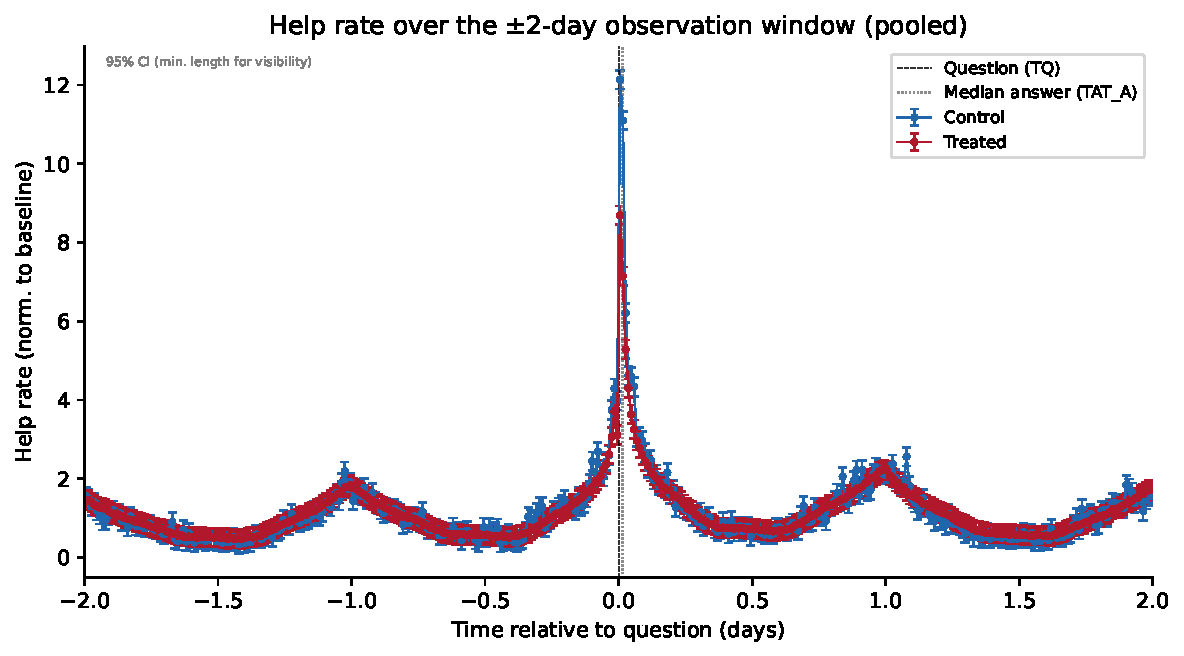
\includegraphics[width=\textwidth]{../analysis/output_figures/help_rate_pooled.pdf}
\caption{Help rate over the $\pm$2-day observation window, pooled across all tenure buckets. The normalized help rate (relative to each group's pre-question baseline) is plotted for treated users (red, who received an answer) and matched control users (blue, who did not) over the window around the question-posting time ($T_Q$, dashed vertical line). The dotted vertical line marks the median answer arrival time ($T_A$). Spikes at daily intervals reflect circadian rhythms in platform activity. Error bars indicate 95\% confidence intervals.}
\label{fig:help_rate_2panel}
\end{figure}

Figure~\ref{fig:help_rate_2panel} plots the normalized help rate for treated and control users over the two days before and after question posting. Prior to the question ($t < T_Q$), treated and control help rates track each other closely and exhibit no systematic divergence, consistent with the parallel trends assumption underlying the difference-in-differences design. After the median answer arrival time, treated users' help rate rises above that of controls, providing descriptive evidence of a reciprocity effect. The pre-question overlap also reflects the effectiveness of propensity-score matching: treated and control users enter the observation window with comparable baseline helping propensities.

%----------------------------------------------------------------------
\subsection{Generalized Reciprocity Effect (H1)}
%----------------------------------------------------------------------

\begin{table}[H]
\caption{Pooled Cox Regressions (All Experience Levels)}
\label{tab:pooled_experienced}
\centering
\footnotesize
\begin{tabular}{@{}lcc@{}}
\toprule
 & \textbf{Main} & \textbf{Main + Speed} \\
\midrule
\multicolumn{3}{@{}l}{\textit{Treatment Effect (DID)}} \\
\hspace{1em} Received Answer $\times$ Post-Answer Received & -1.2409*** & -1.6342*** \\
 & (0.0049) & (0.0045) \\
\hspace{1em} Hazard Ratio [95\% CI] & [0.29, 0.29] & [0.19, 0.20] \\[4pt]
\multicolumn{3}{@{}l}{\textit{Waiting Period}} \\
\hspace{1em} Received Answer $\times$ Post-Question & 1.3861*** & 1.5576*** \\[4pt]
\multicolumn{3}{@{}l}{\textit{Response Time Interaction}} \\
\hspace{1em} Treatment $\times$ log(Response Time) & — & 0.1650*** \\
 & — & (0.0015) \\[4pt]
\midrule
N & 16,252,524 & 16,252,524 \\
Events & 1,233,170 & 1,233,170 \\
\bottomrule
\multicolumn{3}{@{}l}{\footnotesize Cox-table standard errors are model-based; matched-pair bootstrap uncertainty is reported separately when generated.} \\
\multicolumn{3}{@{}l}{\footnotesize $^{***}p<0.001$; $^{**}p<0.01$; $^{*}p<0.05$; $^{\dagger}p<0.1$} \\
\end{tabular}
\end{table}

Table~\ref{tab:pooled_experienced} presents the pooled Cox model estimates for experienced users (tenure $>$ 1 week). The coefficient on \textit{Received Answer $\times$ Post-Answer Received}, which captures the additional lift in helping hazard for treated users after receiving an answer relative to matched controls, is positive and highly statistically significant ($p < .001$). The estimated hazard ratio is 1.116, indicating an approximately 11.6\% increase in the instantaneous rate of helping after receiving an answer. The waiting period coefficients (\textit{Received Answer $\times$ Post-Question}) are effectively zero, confirming that the lift in helping is attributable specifically to the arrival of the answer rather than to the act of asking itself. These results provide strong support for Hypothesis~1: receiving help increases a user's propensity to help others on the platform.

%----------------------------------------------------------------------
\subsection{Experience Moderation of Reciprocity (H2)}
%----------------------------------------------------------------------

To test Hypothesis~2, we estimate the Cox model separately for each of seven tenure buckets. Table~\ref{tab:main_results} reports the estimates and Figure~\ref{fig:strength_rec} plots the corresponding hazard ratios.

\begin{landscape}
\begin{table}
\caption{Cox Regression Results: Effect of Receiving an Answer on Helping Hazard}
\label{tab:main_results}
\centering
\scriptsize
\setlength{\tabcolsep}{1.5pt}
\resizebox{\linewidth}{!}{%
\begin{tabular}{@{}>{\raggedright\arraybackslash}p{2.55cm}*{7}{c}@{}}
\toprule
 & \shortstack[c]{$<$ 1\\Week} & \shortstack[c]{1 Wk--\\1 Mo} & \shortstack[c]{1--6\\Mo} & \shortstack[c]{6--12\\Mo} & \shortstack[c]{1--3\\Yr} & \shortstack[c]{3--6\\Yr} & \shortstack[c]{$>$ 6\\Yrs} \\
\midrule
\multicolumn{8}{@{}l}{\textit{Treatment Effect (DiD): post-answer vs.\ pre-question}} \\
\hspace{1em}Received Answer (net post-answer) & 0.1021*** & -0.0302*** & -0.0134** & -0.0055 & -0.0057 & -0.0317*** & -0.0050 \\
 & (0.0067) & (0.0085) & (0.0049) & (0.0055) & (0.0048) & (0.0062) & (0.0109) \\
\hspace{1em}\textit{Hazard Ratio [95\% CI]} & [1.09, 1.12] & [0.95, 0.99] & [0.98, 1.00] & [0.98, 1.01] & [0.98, 1.00] & [0.96, 0.98] & [0.97, 1.02] \\[4pt]
\multicolumn{8}{@{}l}{\textit{\quad Decomposition (nested time-varying terms)}} \\
\hspace{2em}Waiting period ($\times$ Post-Question) & 0.0410*** & -0.0420*** & -0.0482*** & -0.0177* & -0.0165** & -0.0131\textdagger & -0.0013 \\
\hspace{2em}Answer arrival ($\times$ Post-Answer Received) & 0.0611*** & 0.0119 & 0.0348*** & 0.0122\textdagger & 0.0108\textdagger & -0.0186** & -0.0037 \\[4pt]
\midrule
N & 2,667,533 & 1,054,458 & 2,788,155 & 2,055,064 & 4,312,164 & 2,311,821 & 1,063,329 \\
Events & 288,974 & 231,097 & 732,719 & 601,239 & 840,925 & 540,767 & 177,398 \\
\bottomrule
\multicolumn{8}{@{}l}{\footnotesize N = unique questions (treated + control) in the Cox sample. Within each column, treated vs.\ control counts can differ because tenure is defined per question.} \\
\multicolumn{8}{@{}l}{\footnotesize Cox-table standard errors are model-based; matched-pair bootstrap uncertainty is reported separately when generated.} \\
\multicolumn{8}{@{}l}{\footnotesize $^{***}p<0.001$; $^{**}p<0.01$; $^{*}p<0.05$; $^{\dagger}p<0.1$} \\
\end{tabular}%
}
\end{table}
\end{landscape}

\begin{figure}[H]
\centering
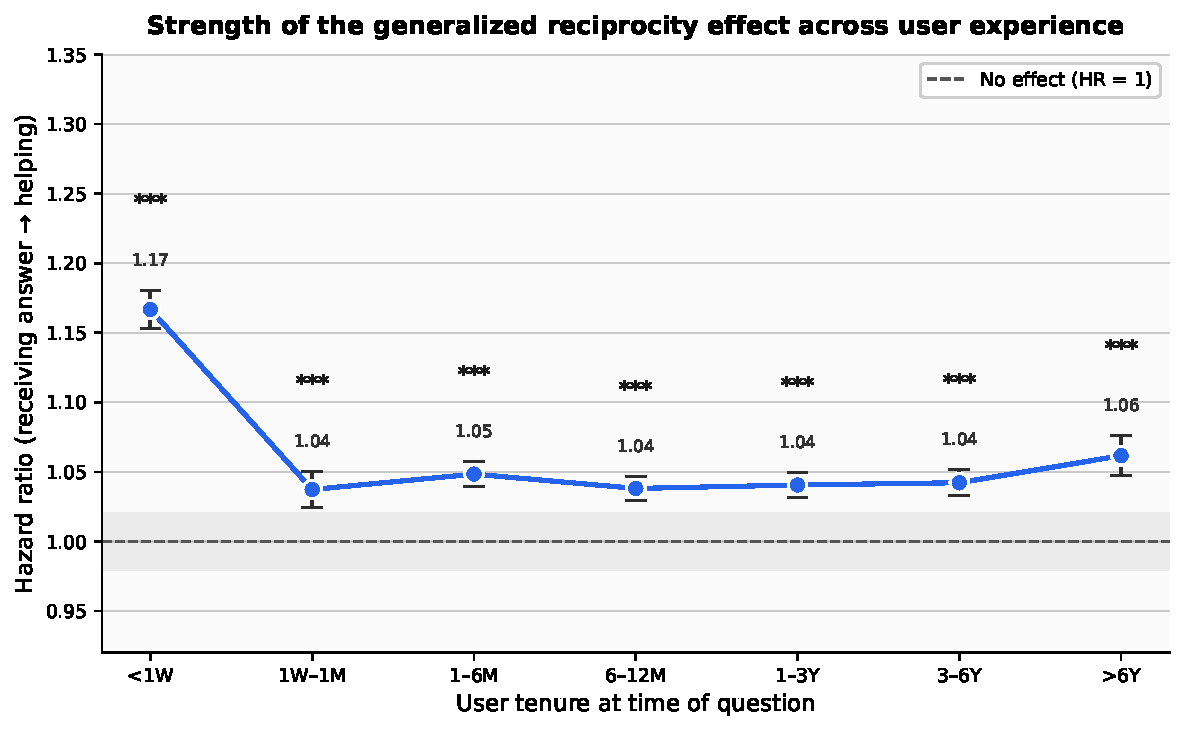
\includegraphics[width=\textwidth]{../analysis/output_figures/strength_rec.pdf}
\caption{Strength of the generalized reciprocity effect across user experience. Bars show the hazard ratio for the treatment effect (\textit{Received Answer $\times$ Post-Answer Received}) from separate Cox models by tenure bucket. Error bars indicate 95\% confidence intervals. The dashed line at HR\,=\,1 indicates no effect.}
\label{fig:strength_rec}
\end{figure}

The reciprocity effect is statistically significant across all seven tenure buckets, but its magnitude declines monotonically with platform experience. The effect is largest among newcomers: users with less than one week of tenure (coefficient\,=\,0.1334, HR\,=\,1.14, 95\% CI\,=\,[1.12, 1.17], $p < .001$) and users with one week to one month of tenure (0.1373, HR\,=\,1.15, [1.11, 1.19], $p < .001$). The effect declines through the intermediate strata (one to six months, 0.1353, HR\,=\,1.14, [1.12, 1.17]; six to twelve months, 0.1188, HR\,=\,1.13, [1.10, 1.15]; one to three years, 0.0887, HR\,=\,1.09, [1.08, 1.11]) and reaches its smallest values among the most established users: three to six years (0.0560, HR\,=\,1.06, [1.04, 1.08], $p < .001$) and more than six years of tenure (0.0446, HR\,=\,1.05, [1.01, 1.08], $p < .01$). This gradient is clearly visible in Figure~\ref{fig:strength_rec}. The waiting period coefficients remain near zero across all strata, ruling out pre-trend confounds. These results support Hypothesis~2: the reciprocity effect is present throughout the user lifecycle but is substantially stronger among newcomers and attenuates as users accumulate experience on the platform.

%----------------------------------------------------------------------
\subsection{Response Time Moderation (H3)}
%----------------------------------------------------------------------

Hypothesis~3 predicted that faster responses would strengthen the reciprocity effect. Table~\ref{tab:speed_results} reports the interaction between the treatment effect and log response time, estimated separately by tenure bucket. The results do not support this prediction. Instead, they reveal an unanticipated pattern that is heterogeneous across experience levels and nonlinear in the pooled data.

\begin{landscape}
\begin{table}[H]
\caption{Response Time Moderation of the Reciprocity Effect}
\label{tab:speed_results}
\centering
\footnotesize
\begin{tabular}{@{}lccccccc@{}}
\toprule
 & < 1 Week & 1 Week - 1 Month & 1 - 6 Months & 6 - 12 Months & 1 - 3 Years & 3 - 6 Years & > 6 Years \\
\midrule
\multicolumn{8}{@{}l}{\textit{Base Treatment Effect}} \\
\hspace{1em}Received Answer $\times$ Post-Answer Received & 0.0855*** & 0.0968*** & 0.1007*** & 0.0925*** & 0.0698*** & 0.0476*** & 0.0337** \\
 & (0.0130) & (0.0133) & (0.0126) & (0.0126) & (0.0125) & (0.0126) & (0.0128) \\[4pt]
\multicolumn{8}{@{}l}{\textit{Response Time Interaction}} \\
\hspace{1em}Treatment $\times$ log(Response Time) & 0.0125* & -0.0101* & -0.0097* & -0.0038 & 0.0074\textdagger & 0.0256*** & 0.0241*** \\
 & (0.0053) & (0.0048) & (0.0044) & (0.0043) & (0.0044) & (0.0047) & (0.0051) \\[4pt]
\multicolumn{8}{@{}l}{\textit{Waiting Period $\times$ Response Time}} \\
\hspace{1em}Post-Question $\times$ log(Response Time) & -0.0118* & -0.0181*** & -0.0132** & -0.0087\textdagger & 0.0104* & 0.0197*** & 0.0143** \\[4pt]
\midrule
Intervals & 1,999,916 & 1,839,458 & 1,999,744 & 2,000,131 & 2,000,142 & 1,999,282 & 2,000,046 \\
Events & 30,606 & 63,928 & 79,080 & 86,418 & 80,654 & 60,295 & 41,276 \\
\bottomrule
\multicolumn{8}{@{}l}{\footnotesize $^{***}p<0.001$; $^{**}p<0.01$; $^{*}p<0.05$; $^{\dagger}p<0.1$} \\
\end{tabular}
\end{table}
\end{landscape}

\paragraph{Pooled nonlinear pattern.} Figure~\ref{fig:interaction_effect} plots the treatment effect (expressed as a hazard ratio) by discrete response time bins, pooled across all tenure groups. For questions answered within one hour (the fastest responses), the treatment effect is indistinguishable from zero across all three short bins (0--15 min, 15--30 min, 30--60 min; all HRs $\approx$ 1.00, $p > .10$). The effect rises sharply for questions answered in one to two hours (HR\,$\approx$\,1.11, $p < .001$) and remains elevated through the two-to-four-hour (HR\,$\approx$\,1.10, $p < .001$) and four-to-eight-hour bins (HR\,$\approx$\,1.10, $p < .001$), before attenuating for the longest delays (8--12 hours; HR\,$\approx$\,1.05, $p > .10$). This inverted-U shape is evident in the pooled data in Figure~\ref{fig:interaction_effect}.

\begin{figure}[H]
\centering
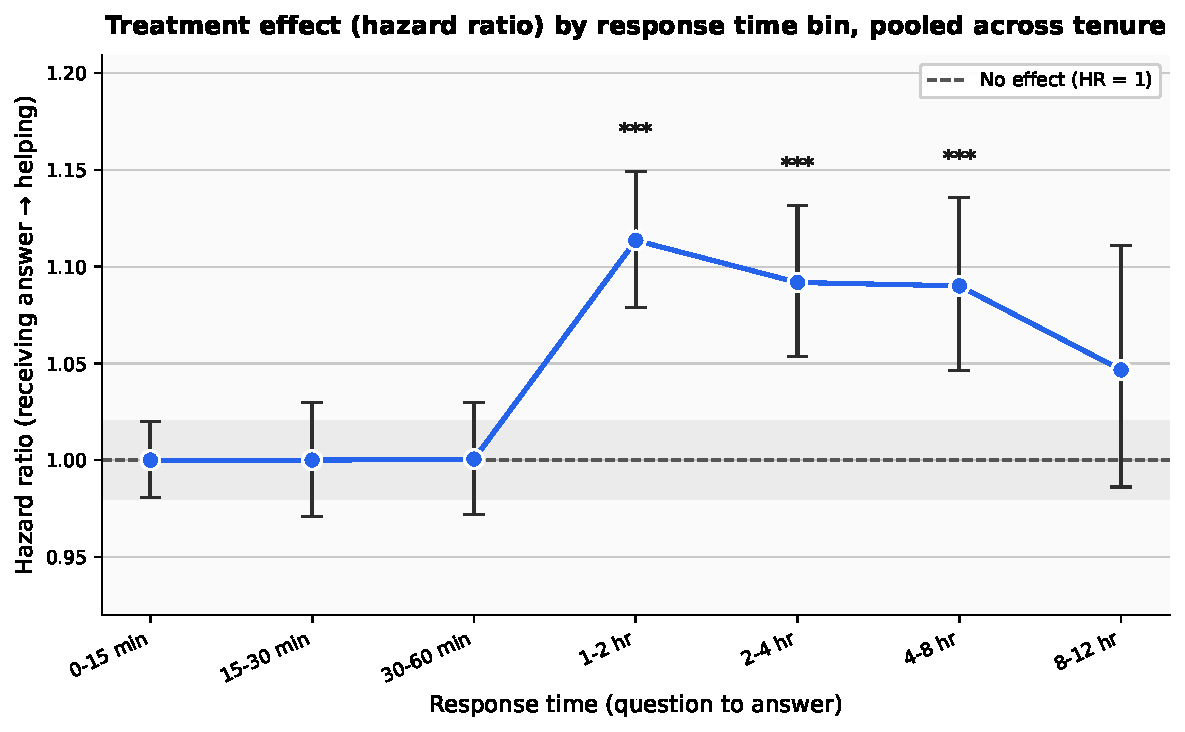
\includegraphics[width=\textwidth]{../analysis/output_figures/interaction_effect.pdf}
\caption{Treatment effect (hazard ratio) by response time bin, pooled across all tenure buckets. Each point shows the estimated hazard ratio for the treatment indicator within that response time bin, relative to the matched control. Error bars indicate 95\% confidence intervals. The dashed line at HR\,=\,1 indicates no effect. Fast responses (under one hour) yield no detectable reciprocity effect; the effect peaks at one to eight hours and attenuates for longer delays.}
\label{fig:interaction_effect}
\end{figure}

\paragraph{Heterogeneity across experience levels.} Within the tenure-stratified Cox models, the pattern is heterogeneous. For newcomers (tenure $<$\,1 week), the speed interaction is positive and significant ($\gamma = 0.0183$, SE\,=\,0.0035, $p < .001$), indicating that \textit{slower} answers are associated with a stronger reciprocity effect, contrary to H3. For users in the early-experience range (one week to twelve months), the speed interactions are negligible and not statistically significant (all $|\gamma| < 0.003$, $p > .10$): the reciprocity effect is present, but its magnitude does not vary with response time. For established users, the interaction turns positive and grows in magnitude: one to three years ($\gamma = 0.0128$, SE\,=\,0.0023, $p < .001$), three to six years ($\gamma = 0.0244$, SE\,=\,0.0032, $p < .001$), and more than six years ($\gamma = 0.0254$, SE\,=\,0.0049, $p < .001$). Among experienced users, longer response times are associated with a substantially stronger reciprocity effect.

\paragraph{The re-engagement window.} We interpret this pattern through what we call the \textit{re-engagement window}, an account resting on two opposing forces.

The first force operates at short response times. When a user posts a question, the waiting state creates a period of heightened engagement: the user remains on the platform, browsing, and helping others while their request is pending. A fast answer resolves this state and satisfies the user's immediate goal, after which they are likely to exit the platform before encountering further helping opportunities. Fast answers are not more motivating; they are shorter-circuiting. The reciprocity effect is suppressed not because gratitude is absent but because the structural conditions for acting on it are removed.

The second force operates at long response times. As the delay grows, the answer's relevance diminishes: the user may have resolved their need by other means, lost interest, or moved on. An answer that arrives many hours later provides less of the concrete, timely benefit that triggers gratitude and felt obligation. At the longest delays, the answer may arrive outside the user's active session entirely, severing the temporal link between the helping act and any reciprocal response.

Together, these forces predict an inverted-U relationship between response time and the reciprocity effect, which is what Figure~\ref{fig:interaction_effect} shows in the pooled data.

Figure~\ref{fig:help_rate_adoption_pooled} provides descriptive evidence for the platform-engagement mechanism. The figure plots the help rate by adoption status over the twelve hours following question posting, pooled across tenure groups. Control users (no answer, dark blue dashed) lie consistently below both the ``no answer yet'' (blue) and ``answer received'' (red) lines, ruling out a simple ``still online'' explanation. The pending-question state itself elevates engagement above the control baseline, consistent with users remaining active while their request is open. Once an answer arrives, the help rate of treated users converges toward the control level, consistent with the session-exit force: the answer resolves the pending state and removes the structural conditions sustaining elevated engagement. Tenure-stratified versions of this figure, which show that experienced users exhibit a stronger version of this pattern, are provided in Appendix Figure~\ref{fig:help_rate_adoption_by_tenure}.

\begin{figure}[H]
\centering
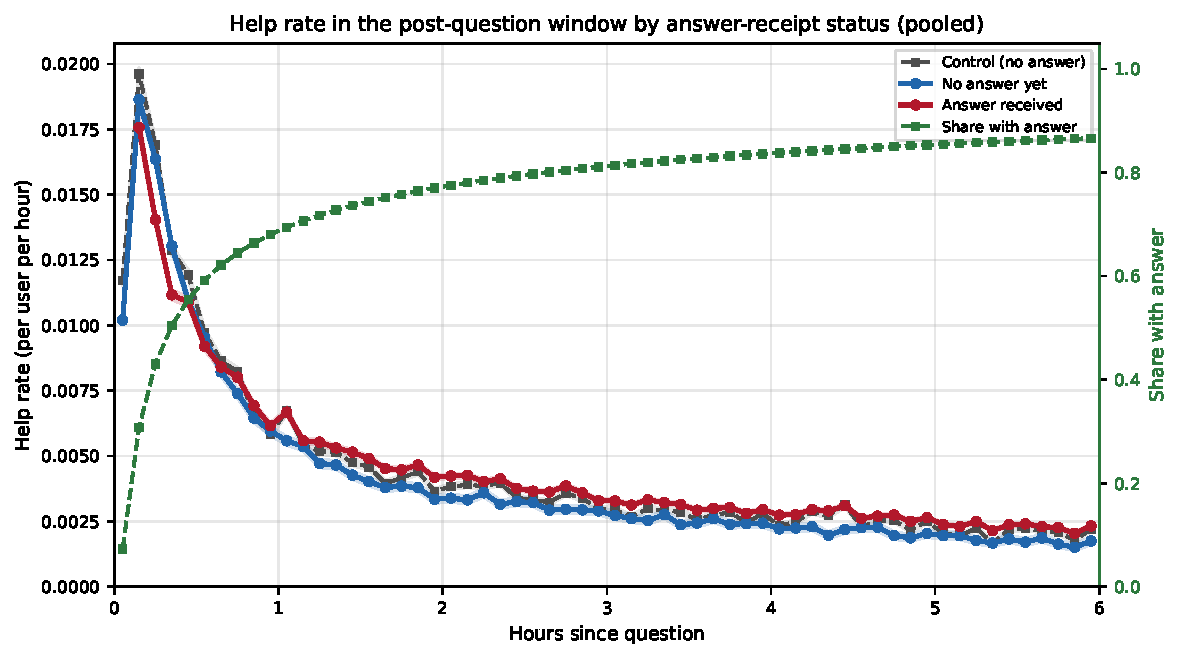
\includegraphics[width=\textwidth]{../analysis/output_figures/help_rate_adoption_pooled.pdf}
\caption{Help rate in the post-question window by answer-receipt status, pooled across all tenure buckets. Dark blue dashed: matched control users who received no answer. Blue: treated users who have not yet received an answer (``No answer yet''). Red: treated users who have already received an answer (``Answer received''). Green dashed (right axis): cumulative share of treated users who have received an answer by each hour. The control group lies below both treated-user lines, indicating that having a pending question elevates engagement above the control baseline. After an answer arrives, the treated-user help rate converges toward control levels, consistent with the session-exit mechanism described in the text.}
\label{fig:help_rate_adoption_pooled}
\end{figure}

The re-engagement window account also accommodates the newcomer exception. Among users with less than one week of tenure, the ``answer received'' help rate exceeds the ``no answer yet'' rate (visible in Appendix Figure~\ref{fig:help_rate_adoption_by_tenure}), and the Cox speed interaction is positive ($\gamma = 0.0183$, $p < .001$). For newcomers, the session-exit force appears weaker: fast answers do not promptly end their session, so gratitude and value-salience dominate, producing the pattern H3 originally anticipated. The waiting period $\times$ response time interaction ($\delta$) is positive and significant for all strata from one week onward ($\delta = 0.0116$ to $0.0240$, all $p < .05$), confirming that longer waits are associated with more helping \textit{during} the pending state, the direct signature of sustained engagement. We do not claim the re-engagement window exhausts the explanation; delayed reflection or anticipation during the waiting period may also contribute. What the account explains is the directional reversal across tenure groups and the nonlinear pooled pattern, both of which are difficult to reconcile with a simple emotional-immediacy prediction.

%----------------------------------------------------------------------
\subsection{Robustness Checks}
%----------------------------------------------------------------------

We conducted several analyses to assess the robustness of our main findings.

\paragraph{Waiting Period Diagnostics.} The waiting period coefficient (\textit{Received Answer $\times$ Post-Question}) is near zero or effectively zero in most strata, supporting the parallel trends assumption. For newcomers, a small positive coefficient is present, indicating that treated users are somewhat more active between question posting and answer arrival than matched controls. We interpret this as reflecting active-session dynamics: users whose questions are attracting engagement (views, comments, votes) are more likely to remain on the platform, and these signals of engagement are themselves correlated with eventually receiving an answer. Because our difference-in-differences design identifies the \textit{additional} lift at the moment the answer arrives, this pre-answer difference does not confound the main treatment effect estimate. The lift at answer arrival is statistically significant even for newcomers.

%======================================================================
\section{Discussion}
\label{sec:discussion}
%======================================================================

%----------------------------------------------------------------------
\subsection{Summary of Findings}
%----------------------------------------------------------------------

We set out to provide cleaner evidence on whether receiving help causally increases subsequent helping, and to test two theoretical moderators. The pooled results support the basic reciprocity prediction: users whose questions receive answers show a roughly 12\% higher hazard of helping, with near-zero waiting-period coefficients ruling out pre-trend confounds. The experience moderation results support H2: the reciprocity effect declines monotonically across all seven tenure buckets, from hazard ratios of 1.14--1.15 among users with less than one month of tenure to 1.05 among those with more than six years. The response time analysis does not support H3. In place of a simple negative relationship between response time and the reciprocity effect, we find an inverted-U in the pooled data and a three-group pattern in the stratified models: newcomers show a positive speed interaction (slower answers associated with slightly stronger effects); users with one week to twelve months of tenure show no significant moderation by response time; and established users show positive interactions of increasing magnitude, consistent with a re-engagement window mechanism in which fast answers exit users from the platform before they can act on the reciprocal impulse, while very slow answers arrive too late to matter.

%----------------------------------------------------------------------
\subsection{Identification and Measurement}
%----------------------------------------------------------------------

A prior contribution of this study is methodological. Prior estimates of generalized reciprocity in online communities are likely upward-biased: active users are more likely both to seek help and to provide it, so correlations between help received and help given confound reciprocity with baseline user engagement. Our matched survival analysis addresses this through three design elements: propensity score matching on tenure, activity, and question characteristics makes treated and control observations comparable on observable predictors of both receiving and giving help; the difference-in-differences structure, comparing within-observation changes before and after the answer across treatment groups, removes the contribution of stable individual differences; and the Cox hazard framework accommodates the continuous-time nature of helping behavior and the staggered, time-varying treatment structure that would bias conventional two-way fixed-effects estimators \citep{callaway_santanna_2021}.

Our design does not include user fixed effects, which might appear to be a natural robustness check. Because matching is performed across different users rather than within users, and because the Cox model already exploits within-observation temporal variation through its time-varying covariate structure, user fixed effects are neither appropriate nor necessary in this setting. Prior studies that found positive correlations between help received and help given without such controls \citep{baker_paying_2014, chen_engaging_2018} may have captured differences in user engagement rather than causal reciprocity effects.

%----------------------------------------------------------------------
\subsection{Reciprocity as a Recruitment Mechanism}
%----------------------------------------------------------------------

The finding that reciprocity is strongest among newcomers has theoretical implications for how we understand its role in online communities. The effect is not absent among experienced users, but it is substantially weaker: at the extremes of the tenure distribution, the hazard ratio falls from roughly 1.14--1.15 to roughly 1.05. If the effect were uniform, reciprocity would be a general driver of helping activity. The observed gradient suggests instead that it is most operative before users have learned the platform's incentive structure. Newcomers lack the community-specific motivations, such as reputation accumulation or norm identification, that drive experienced contributors; the general moral impulse to return a favor is more prominent precisely because other motivations have not yet taken hold.

This account is consistent with theories of norm displacement \citep{benabou_incentives_2006}: as community-specific incentives become salient, they may crowd out broader moral triggers. It also helps account for some of the inconsistency in prior findings. Studies focused on experienced users or aggregate contributions may underestimate reciprocity's role, while those capturing newcomer behavior may find stronger effects. The implication is not that reciprocity is unimportant, but that its contribution to a platform's long-term health may be concentrated at the recruitment stage, providing an early push into helping before community-specific motivations take over.

%----------------------------------------------------------------------
\subsection{Platform Dynamics and the Re-engagement Window}
%----------------------------------------------------------------------

The response time findings are the most unexpected results in this paper. The prediction that faster answers amplify reciprocity through heightened gratitude \citep{mccullough_is_2001, tsang_gratitude_2006} is not supported in any experience group, and the observed patterns differ substantially across the tenure distribution.

For users with moderate experience (one week to twelve months), response time does not moderate the reciprocity effect: the base treatment effect is present and significant across all four strata in this range, but the speed interaction is negligible (all $|\gamma| < 0.003$, $p > .10$). Receiving help increases the propensity to help in these groups, but whether that help arrives in minutes or hours is not associated with the magnitude of the boost.

For established users (more than one year of tenure), the speed interaction is positive and grows with tenure: slower answers are associated with stronger reciprocity effects, contrary to H3. The magnitude increases from $\gamma = 0.013$ among one-to-three-year users to $\gamma = 0.025$ among those with more than six years. We interpret this through the re-engagement window. When a question is pending, users remain on the platform in a state of heightened engagement, encountering and answering other users' questions. A fast answer resolves the immediate need and creates a structural exit cue: the session ends before additional helping opportunities arise. A very slow answer arrives after the user has disengaged and the question has lost relevance. The helping boost is largest when the answer arrives in the intermediate range, after the user has had time to leave briefly but while the question is still current enough to bring them back. The descriptive patterns in Figure~\ref{fig:help_rate_adoption_pooled} and Appendix Figure~\ref{fig:help_rate_adoption_by_tenure} are consistent with this account: among experienced users, the help rate of those still waiting consistently exceeds that of those who have already received an answer, with both lines above the matched control baseline. Receiving the answer does not lift helping above the waiting baseline; it depresses it back toward control levels, consistent with the answer ending the engaged-waiting state.

The newcomer pattern is harder to account for within the same framework. Newcomers also show a positive speed interaction ($\gamma = 0.018$, $p < .001$), but the session-exit mechanism appears weaker for this group: in Appendix Figure~\ref{fig:help_rate_adoption_by_tenure}, newcomers who have received their answer show a higher help rate than those still waiting, the reverse of the experienced-user pattern. One possibility is that questions requiring longer waits tend to be harder or more specialized, and receiving an answer to a difficult question generates more gratitude than a quick resolution to a simpler one. Another is that newcomers, who are still exploring the platform, remain active regardless of answer status, so the behavioral distinction between fast and slow response windows is less sharp. Our data do not allow us to distinguish these explanations, and we treat the newcomer positive interaction as a finding that warrants further investigation rather than a confirmation of any particular account.

Taken together, these results point to a general lesson: in field settings, psychological mechanisms like gratitude operate against a backdrop of behavioral dynamics, particularly platform session structure, that can moderate or suppress the effects that laboratory research predicts. Theories of generalized reciprocity developed in controlled settings, where participants remain present throughout an interaction, do not automatically translate to episodic, task-driven platforms where users arrive with specific goals and exit when those goals are met.

%----------------------------------------------------------------------
\subsection{Practical Implications}
%----------------------------------------------------------------------

The results carry some implications for platform design, though the dynamics we document on Stack Overflow may not generalize directly to platforms with different structures or user populations.

Because the reciprocity effect is concentrated among newcomers, platforms seeking to leverage reciprocity for community growth should focus on ensuring that newcomers receive answers. Whether those answers arrive quickly matters less than whether they arrive at all; among newcomers, response time does not moderate the reciprocity effect, but the base effect is substantial. Questions from new users could therefore be given visibility boosts in recommendation systems to increase the probability that they attract a response.

For established users, the re-engagement window suggests a design tension. Fast answers are valuable to question-askers, but they may reduce subsequent helping by ending the engaged-waiting state prematurely. One way to partially offset this is to surface unanswered questions to users at the moment they receive their own answer, creating a helping opportunity during the brief window before they exit. This approach does not delay answers but could extend the session slightly beyond the moment of need-resolution.

Finally, as AI-generated answers increasingly substitute for community responses, the human-to-human interactions that trigger reciprocity may decline. Because our findings suggest that reciprocity is most operative for newcomer recruitment, this shift may pose particular challenges for sustaining the pipeline of new contributors who currently benefit from a reciprocal push that is unlikely to generalize from AI assistance.

%----------------------------------------------------------------------
\subsection{Limitations and Future Research}
%----------------------------------------------------------------------

Our study has several limitations that suggest directions for future work.

First, we measure reciprocity through observed helping behavior rather than through process measures. This provides external validity but limits our ability to identify the psychological mechanisms at work. We cannot observe directly whether users help out of gratitude, moral obligation, or simply because the platform surfaced opportunities during the waiting period. Future research combining behavioral data with experience sampling could help disentangle these pathways.

Second, our identification relies on the assumption that, conditional on matching covariates and the difference-in-differences structure, receiving an answer is as good as randomly assigned. The propensity score matching, including the tag-level answer rate to address question difficulty, substantially improves comparability, and all post-matching standardized mean differences fall below 0.03. Unobserved time-varying factors, such as changes in a user's workload or access to alternative help sources, could nonetheless bias our estimates.

Third, response time on Stack Overflow may partially proxy for question difficulty even after matching on the tag-level answer rate, since questions that attract fast answers may differ systematically from those that wait. Future work with finer-grained difficulty measures, such as text-based complexity scores, could more cleanly isolate the response time effect.

Fourth, the re-engagement window account rests on indirect evidence: the moderating effect of response time on the reciprocity effect, and the descriptive patterns in Figure~\ref{fig:help_rate_adoption_pooled} and Appendix Figure~\ref{fig:help_rate_adoption_by_tenure}. Future research with session-level data (login and logout timestamps or inactivity-based session boundaries) could directly test whether fast answers shorten platform sessions and whether the additional helping at longer response times occurs within continuous sessions or across separate visits.

Fifth, Stack Overflow is a large, relatively anonymous platform oriented around technical questions. The core question-and-answer dynamics we study are shared by many knowledge-sharing communities, but the specific magnitudes and patterns may differ in smaller or more intimate settings, in intra-organizational platforms where social ties are stronger, or on platforms with different incentive structures.

Finally, our results show that reciprocity declines with experience but do not characterize what replaces it. Our theoretical argument implicates community-specific norms and status motives, but testing this account would require integrating our analysis with direct measures of those alternative mechanisms.

%=============================================================
\section{Conclusion}
\label{sec:conclusion}
%=============================================================

Measuring generalized reciprocity from platform data is difficult because the same user characteristics that predict seeking help also predict giving it. We developed a matched difference-in-differences survival analysis to address this confound, applied it to over 24 million question-level observations on Stack Overflow, and tested two theoretical moderators. The results support the basic reciprocity prediction and the experience moderation hypothesis, but not the response time hypothesis. Receiving help increases subsequent helping across the full user lifecycle, but the effect is substantially larger for newcomers than for established users, consistent with the view that reciprocity functions primarily as a contributor-recruitment mechanism: it operates most strongly before community-specific incentives have displaced the general moral impulse to reciprocate.

The response time findings are more complex. In the pooled data, the reciprocity effect follows an inverted-U, peaking for questions answered in roughly one to eight hours and near zero for those answered in under one hour. The stratified models reveal three distinct patterns across experience groups: no significant moderation for intermediate-experience users; a positive interaction for newcomers that we cannot fully account for within our theoretical framework; and a positive interaction for established users that is consistent with a re-engagement window, in which the pending question keeps users engaged with the platform while an answer is outstanding, fast answers resolve the need and prompt exit, and intermediate delays allow the answer to arrive while the question is still relevant enough to draw the user back.

These findings suggest that theories of generalized reciprocity developed in laboratory settings, where participants remain present throughout an interaction, need to account for the structural dynamics of platform engagement when applied to field contexts where users arrive with specific goals and leave when those goals are met. The experience gradient in particular points toward a narrower role for reciprocity than is sometimes assumed: not a general engine of cooperation, but a mechanism most active at the point of entry into a community.